\section{Results and discussion}
\label{results}
We first describe the raw dataset provided by dermatologists and the one we derived from it, which is more appropriate for evaluation and . Then we describe and explain the experiments and describe the obtained results.\par
\subsection{Datasets Description}
All the data we use in this study was provided by dermatology service of Saint-Etienne hospital under patient consent. This data contain three modalities of images: Clinical Photography, Dermatoscopy and \ac{rcm}. Each of these modalities is acquired by a specialist. Furthermore, each patient is associated to a ground truth label from histopathology \cite{Cinotti2018}.\par
In this work, we focus only on the \ac{rcm} images and Lentigo pathology parts of this dataset. Images related to this imaging modality are acquired into the dermoepidermal junction, considered by specialist as relevant for diagnosis of Benign Lentigo and Malignant Lentigo. The depth of acquisition nor the spatial location information are not available. Processed \ac{rcm} images from this dataset have spatial resolution of 1000 by 1000 pixels, with a quantification on a single channel on 1 byte.\par
As our goal is to provide a classification over images, we build a new dataset with an annotation on each image, with the help of a specialist. This dataset contain 2098 \ac{rcm} annotated images related to 60 patients. The same three types of labels as previously have been assigned: “Malignant” label for images including at least malignant information, “Benign” label for images being composed of benign pathology and finally a “Healthy” label corresponding to absence of Malignant and Benign characteristics. In further references, we will consider it as our “Original images”.\par
\begin{figure}[H]
\centering
    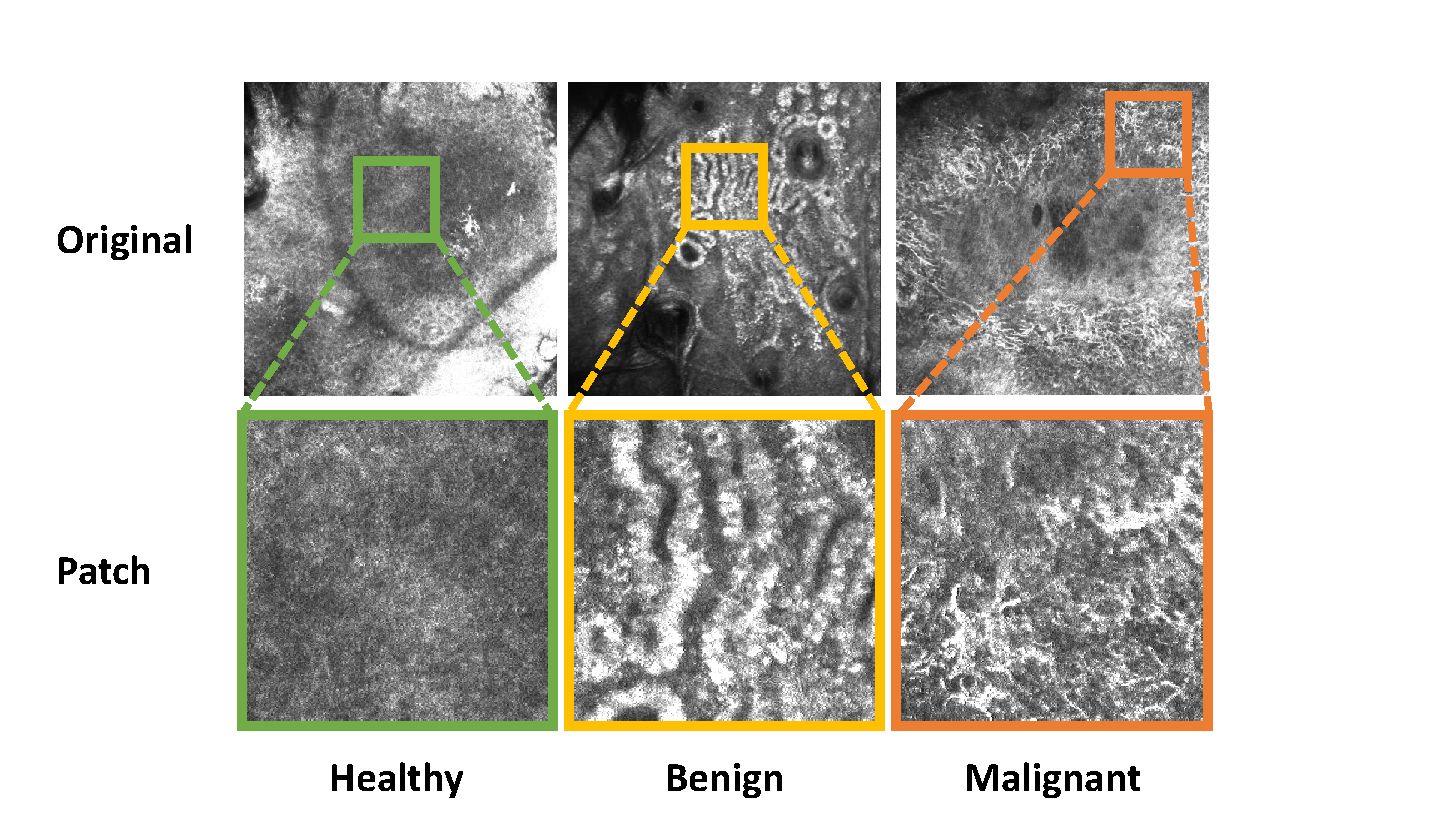
\includegraphics[width=0.9\linewidth]{content/figures/Data.pdf}
    \caption{Examples of full images and extracted patches from skin dermal-epidermal junction with \ac{rcm}.}
    \label{data}
\end{figure}
Despite of these annotations, an image may contain malignant, benign or both tissues. In addition and for this particular work, we built with guidance of a specialist another subset of data containing images with a single type of tissue. These new data consist of thumbnails with a spatial resolution of 250 by 250 pixels. A total of 2307 thumbnails are extracted belonging to the three previous categories, with respectively 259 healthy images, 1622 benign images and 426 malignant images (see \Cref{data} for extraction example). In the next part of this paper, we will make reference to these data as “Thumbnails”.
\subsection{Results and Analysis}
Our validation protocol remains the same for each experiment: a nested cross validation is used, known to be less biased than simple cross validation way \cite{Cawley2010}. This process allows to cross validate hyperparameters and evaluate objectively prediction models. Each of the cross-validation steps is based on K-Fold strategy with k=5 in our case. For this purpose we use of “Scikit Learn” library for Machine Learning classification, validation and metric~\cite{pedregosa2011scikit}.\par
We evaluate our experiments using F1-Score metric, as it is statistically suitable for unbalanced populations and provide information about recall and precision. In addition, a standard deviation is calculated to achieve an analysis of the stability of models along nested cross validation.\par
\begin{table}[h]
\centering
    \begin{tabular*}{\linewidth}{l@{\extracolsep{\fill}}ll}
        \hline
        \textbf{Methods} & \textbf{Original images} & \textbf{Thumbnails}\\
        \hline
        Wavelets & 0.45$\pm$0.07 & 0.59$\pm$0.05\\
        \hline
        Haralick & 0.49$\pm$0.09 & 0.61$\pm$0.07\\
        \hline
        Transfer Learning (Max Pool) & 0.57$\pm$0.04 & \textbf{0.89$\pm$0.03}\\
        \hline
        Transfer Learning (Avg Pool) & \textbf{0.66$\pm$0.04} & \textbf{0.89$\pm$0.03}\\
    \end{tabular*}
    \caption{Comparison of feature extraction methods for three classes classification using F1-Score on original images and thumbnails.}
    \label{simple_scores}
\end{table}
In \Cref{simple_scores}, we first achieve a comparison over the two handcrafted feature extraction methods, and Transfer Learning methods using “Global Maximum Pooling” and “Global Average Pooling”. In both cases when considering the whole image or when using thumbnails, Transfer Learning methods significantly overtake handcrafted methods (largest score for F1-Score and smallest standard deviation value). Inter-comparison of Transfer learning methods show that the results are similar for MAX and AVG pooling for Thumbnails. However,  when using the entire image, Average Pooling performs better than MAX pooling. This result may be explained by the fact that the activation map is not reduced to a single value as it is the case of Max-Pooling. \par
\begin{table}[h]
\centering
    \begin{tabular*}{\linewidth}{l@{\extracolsep{\fill}}lll}
        \hline
        \textbf{Methods} & \textbf{H vs B vs M} & \textbf{H vs L} & \textbf{NM vs M}\\
        \hline
        Decision level& 0.53$\pm$0.04 & 0.69$\pm$0.03 & 0.70$\pm$0.02\\
        \hline
        Decision level + Overlap & 0.59$\pm$0.01 & 0.71$\pm$0.01 & 0.76$\pm$0.02\\
        \hline
        Score level& 0.69$\pm$0.03 & 0.73$\pm$0.02 & 0.82$\pm$0.02\\
        \hline
        Score level + Overlap & \textbf{0.73$\pm$0.03} & \textbf{0.76$\pm$0.02} & \textbf{0.85$\pm$0.02}\\
    \end{tabular*}
    \caption{Comparison of sliding window methods based on decision or prediction scores and impact of an overlap of half of size through decision.}
    \label{sliding_scores}
\end{table}
Since the best results (in \Cref{simple_scores}) are obtained by use of the Transfer Learning with “Global Average Pooling”, we use it as feature extraction method in next experiments. \Cref{sliding_scores}, provide results of second pipeline (using a sliding window as a way to extract patches over the original \ac{rcm} images. We consider also an overlap between thumbnails of half of their size. The scores obtained for patches are merged later to make a decision (see \Cref{detection} example of low level decisions). This table include comparison over three labels classification and binary classification by performing “Healthy” vs “Lesional” (H vs L) and “Non Malignant” vs “Malignant” (NM vs M). Sliding window prediction based on scores is much more efficient than using simple decisions and seems intuitive as we get more information to explain a single label. Also, the use of an overlap slightly improved classification results in both “Decision level” and “Score level”.\par
\begin{figure}[h]
    \begin{center} 
        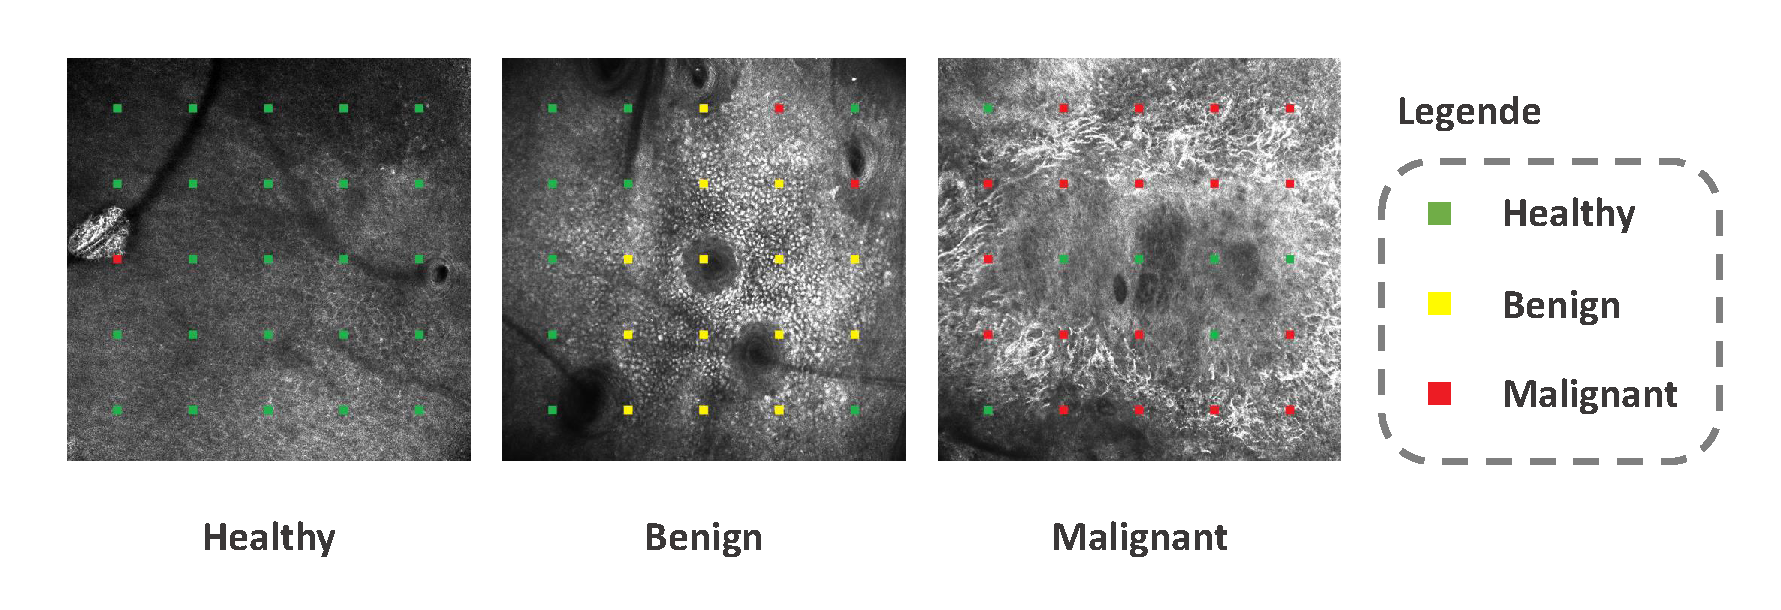
\includegraphics[width=\linewidth]{content/figures/Detection.pdf}
        \caption{Exemple of sliding window performed on full images to reach some local decisions.}
        \label{detection}
    \end{center} 
\end{figure}
Furthermore, this last table shows also that classification of “Non Malignant” against “Malignant” pathologies are much more significant than classification of “Healthy” against “Pathological” and can be due to similarity in patterns between “Healthy” and “Benign” tissues. However, this can be useful in a clinical context as their objectives are to detect malignant pathologies on patients.
